\documentclass[11pt,twoside,a4paper]{article}

\usepackage{graphicx,lmodern,hyperref,calc,enumitem}
\usepackage[T1]{fontenc}
\usepackage[margin=1in]{geometry}

\begin{document}

\title{Computing Linux Project\\
a452}
\author{Chris Hobbs}
\date{May, 2015}
\maketitle

In this task, I will be exploring the linux commandline, and explaining the processes needed to perform some basic actions with the commandline.

\section{A \emph{prompt} introduction.}

Here is the default prompt on debian linux computers:\\

\includegraphics{prompt}

This prompt shows some important information to the user about the current environment that the computer is working in so that the user is able to make decisions on what to do. The prompt is made up of the following parts:
\begin{itemize}
  \item The current user (the part before the at-sign),
  \item The hostname of the current computer (the part between the at-sign and the colon), and
  \item The current directory (the part between the colon and the pound sign).
\end{itemize}

The current directory is shown in this example by the tilde character, which means that you are in your home directory (/home/username). The at-sign was chosen because it reflects the fact that the user is `at' the computer with the shown hostname. In the early internet, it was very likely that the user-hostname pair was actually the user's email.

\section{\emph{ls}ting files.}

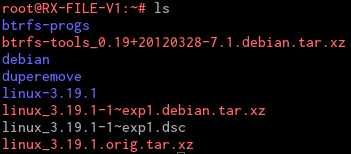
\includegraphics{ls}

When you type \verb|ls| then press enter, you are executing the ls command. A command is simply a program which does something. They typically have short, easy to type names for convenient use at a terminal.

The ls command in the POSIX specification (which linux conforms to), is used to list the contents - in terms of files and folders - of a directory. When used without any arguments, it lists the current directory.

\pagebreak
The output of ls is colourised, with each colour having a different meaning:\cite{ls-colours}
\begin{description}[leftmargin=!,labelwidth=\widthof{\bfseries Light Blue}]
  \item[Blue] directory
  \item[White] unknown file
  \item[Green] executable
  \item[Light Blue] link
  \item[Pink] image
  \item[Red] archive
\end{description}

\section{Playing with \emph{pipes}.}

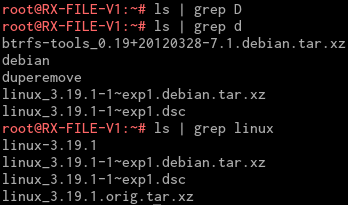
\includegraphics{ls-grep}

The vertical bar character is used on the commandline to pipe the output of one command into the input of another. For this reason it is commonly called the pipe character. For the \verb!ls | grep D! example, we are piping the output of \verb|ls| (a listing of the current directory) into the \verb|grep| command, which searches the data from ls for the character `D'.

\newpage
\begin{thebibliography}{9}

\bibitem{ls-colours}
  karthick87,
  \emph{What do the different colors mean in the terminal?},
  Ask Ubuntu,
  http://askubuntu.com/a/17300

\end{thebibliography}

\end{document}